\documentclass[english]{article}
% \usepackage{babel}
% \usepackage[hyperref=true,style=ieee]{biblatex}  % biblatex reference macro package
% \addbibresource{ref.bib}  % Add reference bib source
\usepackage{lipsum}  % Import macro package for generating paragraphs
% \usepackage{ctex} % Add ctex macro package to support Chinese
\usepackage{graphicx} % Load graphics processing macro package
\usepackage{booktabs} % For beautifying table lines
\usepackage{caption} % For adding table titles
\usepackage{float}
\usepackage{tabularx}
\usepackage{tcolorbox}
\usepackage{enumitem} % 用于调整列表格式
\tcbuselibrary{listings}
\usepackage{array}
\usepackage[dvipsnames]{xcolor}
\usepackage{tikz}
\usepackage{hyperref} 
% \usepackage{tocbibind}
\usetikzlibrary{positioning} % Load positioning library
\renewcommand{\refname}{References}

\hypersetup{
    colorlinks=true, % Use colors instead of borders
    linkcolor=black, % Link color is black
    citecolor=black, % Citation color is black
    urlcolor=blue    % URL color is blue (can be modified as needed)
}
\lstset{
 basicstyle=\ttfamily, % Set font family
 breaklines=true, % Automatic line wrapping
 keywordstyle=\bfseries\color{NavyBlue}, % Set keywords to bold, color is NavyBlue
 morekeywords={}, % Set more keywords, separated by commas
 emph={self}, % Specify emphasized words, separated by commas if multiple
    emphstyle=\bfseries\color{Rhodamine}, % Emphasized word style
    commentstyle=\itshape\color{black!50!white}, % Set comment style, italic, light gray
    stringstyle=\bfseries\color{PineGreen!90!black}, % Set string style
    columns=flexible,
    % numbers=left, % Display line numbers on the left
    % numbersep=2em, % Set the position of line numbers
    % numberstyle=\footnotesize, % Reduce line numbers
    frame=single, % Border
    framesep=1em, % Set the distance between code and border
	tabsize=2, % Set tab width to 2 spaces
    showstringspaces=false, % Do not show spaces in strings
}

\usepackage[margin=1in]{geometry}
\title{\textbf{ztest}: A Fast, User-Friendly, Lightweight C++ Unit Testing Framework}
\begin{document}
\maketitle
\tableofcontents  % Generate table of contents
\newpage
\section{Requirement Analysis for System}% Requirement Analysis
\subsection{The Background and Motivation of System}
% As our coding abilities progress, it becomes increasingly essential to practice the skills required for constructing C++ programs. Consequently, our team has devised a plan to develop a highly user-friendly note-taking system. This system is envisioned to support a wide array of note styles, with Markdown being one of the prominent ones. It will offer users the flexibility to express their thoughts and record information in the format that suits them best. Additionally, a built-in calendar function will be incorporated to present the daily schedule. Moreover, a comprehensive file management system is also on the cards. The combination of these features is set to make our note-taking system a go-to tool for individuals seeking an efficient and versatile digital workspace.
With the increasing demand for complex system architecture design capabilities, mastering object-oriented design principles and pattern-based engineering practices has become a core goal of advanced software engineering education. This not only requires understanding the dynamic collaboration between classes and objects, but also the ability to solve architectural challenges using design patterns and abstract thinking.
Existing unit testing frameworks (such as Google Test) have several drawbacks, including a steep learning curve, limited concurrency support, overly simplistic reporting systems, and average extensibility. Our team plans to develop a flexible, efficient, and easy-to-use (with a graphical user interface, GUI) testing tool. The goal is to provide an intuitive and user-friendly environment for developers and testers to write, run, and manage test cases. The tool will support various types of tests (such as unit tests and integration tests) and provide detailed test result reports.
\begin{table}[h]
    \centering
    \caption{Comparison of Mainstream Testing Frameworks}
    \label{tab:compare}
    \begin{tabularx}{\textwidth}{lXXXX}
        \toprule
        \textbf{Framework}  & \textbf{GUI Support} & \textbf{Concurrency} & \textbf{Reporting} & \textbf{Extensibility} \\
        \midrule
        Google Test (C++)   & None                 & Limited              & Basic              & Medium                 \\
        JUnit (Java)        & Eclipse Plugin       & Supported            & HTML/XML           & High                   \\
        PyTest (Python)     & Third-Party Tools    & Excellent            & Rich               & Excellent              \\
        Catch2 (C++)        & None                 & Average              & Simple             & Medium                 \\
        \textbf{Ours} (C++) & Yes                  & Excellent            & Rich               & High                   \\
        \bottomrule
    \end{tabularx}
\end{table}
\subsection{System Objectives}% System Objectives
% A note-taking system with a user-friendly UI supporting markdown format. We use xmake for the management of the entire project and imgui for UI design, introducing glew, cmark dynamic link libraries, and the OpenGL library. We use "xmake b" for compiling and "xmake r" for running.
% This is a note-taking system with a user-friendly interface that supports Markdown format. We use xmake to manage the entire project and ImGui for UI design, while introducing GLEW, cmark dynamic link libraries, and the OpenGL library. Additionally, we use the "xmake b" command for compilation and the "xmake r" command to run the program.
% \section{System Features}
The design goal of this testing framework is to provide a flexible, efficient, and easy-to-use (with a graphical user interface, GUI) testing tool that supports test case management, assertion validation, test execution, and result reporting. The following sections detail its features in terms of test case management, assertion mechanisms, test executor, and result reporting.

\subsubsection{Test Case Management}
Test case management is one of the core functions of the testing framework, supporting the definition, registration, and organization of test cases. Test cases can be defined through inheritance from a base class or using a factory pattern, and support for setting up pre-test and post-test hook functions is provided.

\paragraph{Creating Individual Test Cases}
Three methods for creating test cases have been implemented: chain creation, macro definition, and inheritance definition:

\begin{enumerate}
    \item \textbf{Chain Creation}: Through chain creation, customized test cases can be achieved. In network programming tests, using chain creation aligns more logically with the requirements. An example is provided below:
          \begin{lstlisting}[language=C++]
auto test_case = TestFactory::createTest("Add", ZType::Z_SAFE, "", add, 2, 3)
                 .setExpectedOutput(5)
                 .beforeAll([]() { logger.info("Init\n"); })          
                 .afterEach([]() { logger.info("Clean\n"); }).build();
                \end{lstlisting}
    \item \textbf{Macro Definition}: Through macro definition, customized test cases can be achieved. Macro definitions greatly simplify the syntax, making test case definitions clearer and more structured. The actual implementation is inheritance definition + automatic registration.
          \begin{lstlisting}[language=C++]
ZTEST_F(BasicMath, FailedAdditionTest) {
    EXPECT_EQ(6, add(2, 3));
    ASSERT_TRUE(6==add(2, 3));
    return Zstate::Z_SUCCESS;// If this point is reached, the test is successful
}
                \end{lstlisting}
    \item \textbf{Inheritance Definition}: By inheriting from the test base class, customized test cases can be achieved with higher extensibility, allowing for the definition of more custom test methods.
          \begin{lstlisting}[language=C++]
class MathTests_Addition : public ZtestBase {
    public:
        MathTests_Addition() : ZtestBase("MathTests.Addition", ZType::ZSAFE, "Test addition function") {}
        Zstate run() override {
                EXPECT_EQ(5, add(2, 3)); // Expected result is 5
                EXPECT_EQ(0, add(0, 0)); // Expected result is 0
                return Zstate::Z_SUCCESS;
        }
};
\end{lstlisting}
\end{enumerate}
\paragraph{Test Case Registration} In the case of macro definitions, the \textbf{ZTestRegistry} test registration center can be used to dynamically register test cases. For inheritance from the test base class, due to the higher degree of freedom given to users, for safety reasons, users are required to register manually. For chain-created test cases, registration can be achieved by calling the registration function after build, or by manual addition.
Here is an example of using the test registration center class:
\begin{lstlisting}[language=C++]
// Manual registration example
ZTestRegistry::getInstance().registerTest(std::make_shared<MathTests_Addition>());
\end{lstlisting}
\paragraph{Building Test Suites}
Multiple test cases can be organized through the \textbf{ZTestSuite} class, supporting batch execution and multi-threaded testing. It also records the time required to run multiple test cases, the number of test cases passed, and other metrics.

\begin{lstlisting}[language=C++]
auto mathSuite = std::make_unique<ZTestSuite>("Math", ZType::Z_SAFE,"math test");
// Add individual test cases to the suite
mathSuite->addTest(TestFactory::createTest("Addition", ZType::Z_SAFE, "", add, 2, 3).setExpectedOutput(5).build());
mathSuite->addTest(TestFactory::createTest("Subtraction", ZType::Z_SAFE, "", subtract, 5, 3).setExpectedOutput(2).build());
\end{lstlisting}



\subsubsection{Assertion Mechanisms}
Assertion mechanisms are used to validate whether the expected results of test cases are correct. The framework provides a variety of assertion macros, such as \textbf{EXPECT\_EQ} and \textbf{ASSERT\_TRUE}, to quickly validate conditions within tests.
The main assertions provided are:
\begin{itemize}
    \item \textbf{EXPECT\_EQ}: Verifies whether two values are equal.
    \item \textbf{ASSERT\_TRUE}: Verifies whether a condition is true.
\end{itemize}
Usage examples are as follows:
\begin{lstlisting}[language=C++]
// If the assertion fails, an exception is thrown
EXPECT_EQ(5, add(2, 3));
ASSERT_TRUE(6==add(2, 3));
\end{lstlisting}

If an assertion fails, a \textbf{ZTestFailureException} exception is thrown. Additionally, by inheriting from the \textbf{ZTestFailureException} exception handling function, custom exception handling logic can be defined.


\subsubsection{Test Executor}
The test executor is responsible for managing the execution of test cases, supporting \textbf{multi-threaded} parallel execution of test cases, and collecting test results. It implements automatic scheduling of tests and statistical analysis of test results.

The \textbf{ZTestContext} class is used for test context management, responsible for maintaining the test case queue and executing tests in parallel using multiple threads.
\begin{lstlisting}[language=C++]
// Define a test context object
ZTestContext context;
// Add test cases to the test queue
for (auto &&test : registeredTests) 
    context.addTest(std::move(test));
// Execute test cases in parallel using multiple threads
context.runAll();
\end{lstlisting}

Two types of test cases can actually be defined: \textbf{z\_safe} and \textbf{z\_unsafe}. These two types correspond to two testing modes. \textbf{z\_safe} test cases are thread-safe, while \textbf{z\_unsafe} test cases are not thread-safe. The default type is \textbf{z\_safe}. If \textbf{z\_unsafe} types appear during testing, the framework will wait for their execution to complete before running \textbf{z\_safe} test cases.

\subsubsection{Result Reporting}
After testing is completed, the framework generates a detailed test result report, including test names, execution time, pass/fail status, and error information.
We define three states for test results:
\begin{itemize}
    \item \textbf{z\_success}: Test passed.
    \item \textbf{z\_failed}: Test failed.
    \item \textbf{z\_unknown}: Test not completed.
\end{itemize}
\textbf{Logging} Test results are output through the \textbf{ZLogger} class to the console or \textbf{a file}.
The output rules are as follows:
[   info   ] indicates test information, [   FAILED  ] indicates test failure, and [   OK   ] indicates test success.
An example output is as follows:
\newpage

\begin{lstlisting}[language=C++]
    [    OK    ] BasicMath.NegativeTest (0 ms)
    [   info   ] Preparing environment for addition test...
    [    OK    ] Advanced.Multiplication (0 ms)
    [  FAILED  ] BasicMath.FailedSubtractionTest (1 ms)
    Error: Test Failure in BasicMath.FailedSubtractionTest:
      Expected: 3
      Actual  : 2
    [  FAILED  ] BasicMath (1 ms)
\end{lstlisting}
The \textbf{ZTestResult} class also saves information such as test execution time, pass/fail status, and error messages to store test results.
\subsubsection{GUI Display}
Test results can be displayed through a GUI. Future plans include adding functionality to the GUI interface for adding, deleting, modifying test cases, and exporting test reports. The general interface design is shown in the figure below.
\begin{figure}[H]
    \centering
    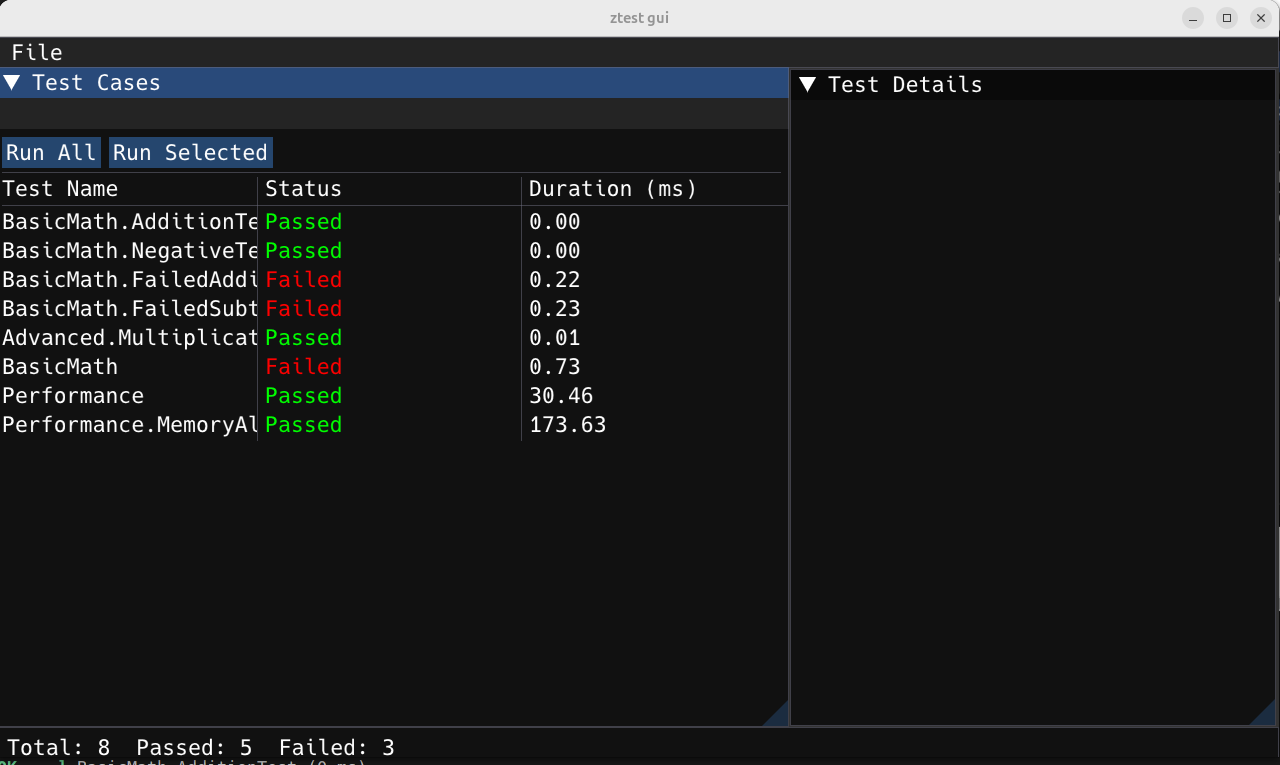
\includegraphics[width=\textwidth]{img/gui.png}
    \caption{Test Management Interface Layout}
    \label{fig:gui}
    \small
\end{figure}

% \section{Technical Selection}
% \begin{table}[H]
%     \centering
%     \caption{Development Environment Configuration}
%     \begin{tabular}{@{}lc@{}} % Remove extra spacing on the left and right of the table
%         \toprule
%         \textbf{Component} & \textbf{Tool Used for Development} \\
%         \midrule
%         Compiler           & Clang                              \\
%         Graphics API       & OpenGL                             \\
%         GUI Framework      & Dear ImGui                         \\
%         Markdown Parser    & cmark                              \\
%         Server             & Python, Flask                      \\
%         Upload Tool        & libcurl                            \\
%         Plugin System      & Lua/Python                         \\
%         PDF Generation     & Pandoc                             \\
%         Build System       & XMake                              \\
%         \bottomrule
%     \end{tabular}
% \end{table}
% \subsection{GUI Framework}
% Many existing C++ markdown note-taking software applications use the QT framework, such as vnotex/vnote and nuttyartist/notes. The reason for selecting this framework is that the qt webengine in the QT library can conveniently use the encapsulated Chromium to render markdown.
% However, this solution has issues such as large compiled file sizes and an overly bloated framework. As a senior programming course project, using this highly encapsulated technology is too simple and does not help in understanding advanced programming techniques.

% Therefore, we decided to use the imgui framework. Compared to QT, this framework has the advantages of being lightweight, efficient, and highly customizable. Although this framework is popular in the open-source community, no markdown note-taking software has been developed using it yet. Thus, its significance is much greater than redeveloping a relatively mature QT note-taking software. From a learning perspective, using this framework allows us to gain a deeper understanding of the underlying implementation of GUI frameworks.
% \subsection{Build System}
% Considering the high learning curve and redundant, cumbersome syntax of cmake, we decided to use xmake as the build system.
% Xmake is a lightweight cross-platform build tool based on Lua. Using the xmake.lua file to maintain project builds, its configuration syntax is more concise and intuitive compared to makefile/CMakeLists.txt. It is very friendly to beginners and allows us to focus more on actual project development within a short time.
% \subsection{Markdown Parsing}
% Since markdown parsing is part of the content of a compilation principles course, we believe that re-implementing it in this course would not be very meaningful. Therefore, we chose the cmark tool to parse markdown source code into an AST (Abstract Syntax Tree).
% \subsection{Server}
% The implementation of the cloud server is not the core of this tool, so we used Python and the Flask library for a simple implementation. In fact, it could be replaced with a server written in C++ (if any group has implemented server-side code, cooperation is possible).

% However, the communication between the local machine and the server uses libcurl (a C++ library). Libcurl is a widely used, open-source client URL transfer library that supports multiple protocols and provides many APIs for data transfer, such as file transfer, FTP, HTTP, HTTPS, SMTP, etc.

% \subsection{Plugin System}
% Implemented using dynamic library linking in C++. On Linux, it is realized using dlfcn.h. Future plans include implementing plugins using Lua or Python.
\newpage
\section{Overall Architecture}
The core module loads test cases and functions to be tested through a plugin mode. The core module is divided into four parts.
\begin{figure}[H]
    \centering
    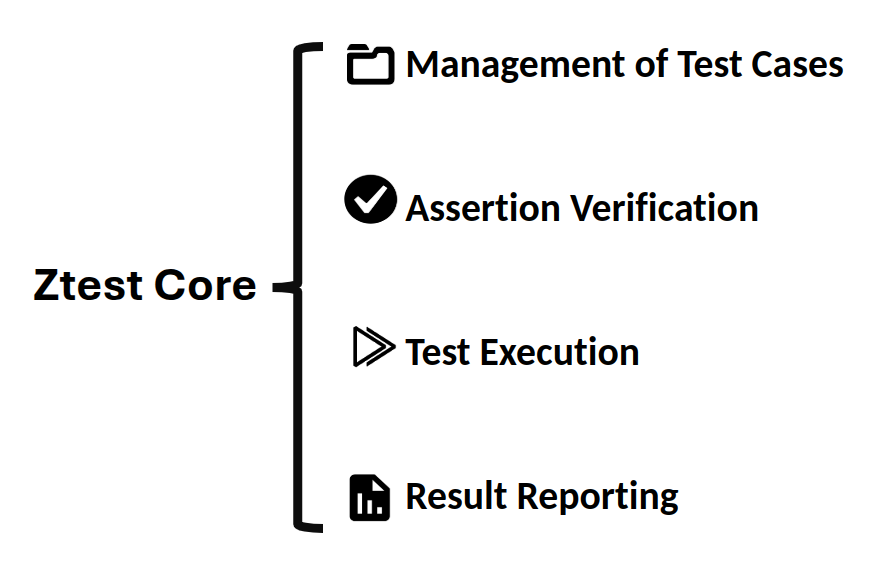
\includegraphics[width=0.6\textwidth]{img/ztest.png} % Insert image
    \caption{ ztest core architecture}
    \label{fig:ztest core architecture}
\end{figure}

The GUI architecture uses the MVC (Model-View-Controller) pattern. The View focuses on the UI that users see and provides interaction. The Controller acts on the model and view. It controls the flow of data to model objects and updates the view when data changes. It separates the view from the model. The Model mainly implements the modeling of underlying files.
\begin{figure}[H]
    \centering
    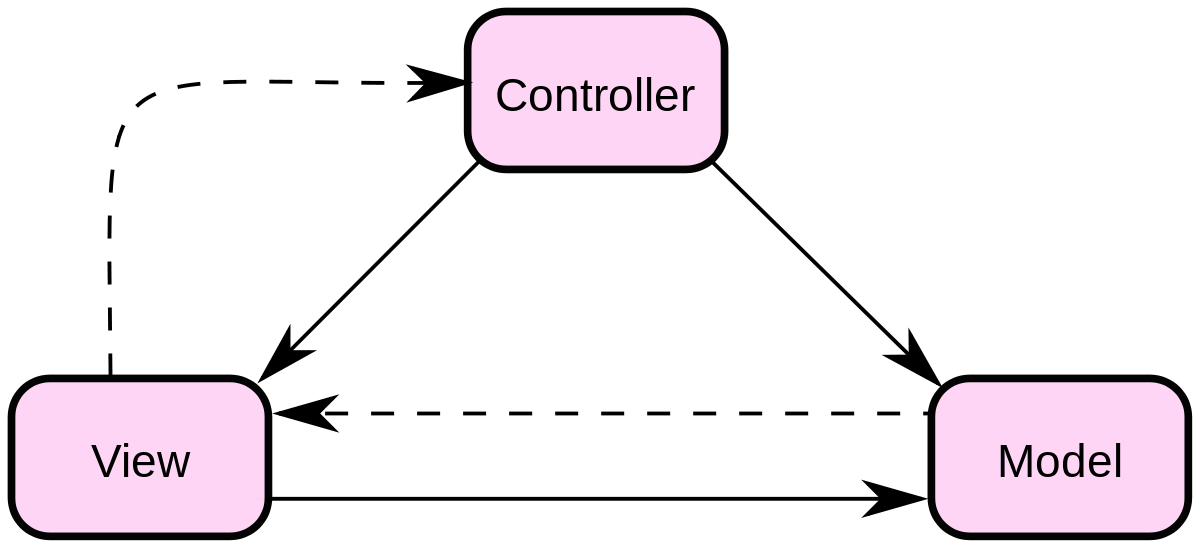
\includegraphics[width=0.6\textwidth]{img/mvc.png} % Insert image
    \caption{ ztest gui architecture}
    \label{fig:mvc}
\end{figure}
\section{Program Analysis}

\subsection{Technical Details}
\subsubsection{Testing Framework Design}

\begin{itemize}
    \item \textbf{ZtestInterface}: Defines the basic interface for test cases, including methods for obtaining test names, running tests, and getting test types.
    \item \textbf{ZtestBase}: Serves as the base class for test cases, implementing basic attributes and methods for tests, such as test names, test types, description information, pre-test hook functions (beforeAll), and post-test hook functions (afterEach).
    \item \textbf{ZtestSingleCase}: Inherits from \textbf{ZtestBase} and is used to define individual test cases. It supports setting test functions, expected results, and description information, and implements the logic for executing tests.
    \item \textbf{ZTestSuite}: Used to organize multiple test cases, supporting batch execution of tests and statistical analysis of test results (passed, failed, total time taken, etc.).
    \item \textbf{ZTestRegistry}: Implemented using the Singleton pattern, this test registration center is responsible for registering and managing test cases, supporting dynamic addition of test cases.
    \item \textbf{ZTestContext}: The test context management class is responsible for maintaining the test case queue and executing test cases in parallel using multiple threads, while also collecting and managing test results.
\end{itemize}
\subsubsection{Test Case Construction and Execution}
The construction of test cases is implemented through the \textbf{TestBuilder} class, supporting chain calls to set test functions, expected results, pre-test hooks, and post-test hooks. The \textbf{TestFactory} class provides convenient methods for creating test cases.

During test execution, the \textbf{ZTestContext} class retrieves test cases from the test queue and uses the \textbf{ZTimer} class to time the tests, recording the start time, end time, and duration of each test. Test results are encapsulated in the \textbf{ZTestResult} class, and detailed information about test results is output to the console.

\subsubsection{Assertions and Exception Handling}
The framework provides assertion macros \textbf{EXPECT\_EQ} and \textbf{ASSERT\_TRUE} to compare expected values with actual values or to verify whether conditions are true. If an assertion fails, a \textbf{ZTestFailureException} exception is thrown, and error information is recorded.

\subsubsection{Test Suites and Multi-threaded Execution}
Test suites (\textbf{ZTestSuite}) can contain multiple test cases and support batch execution. The test context (\textbf{ZTestContext}) executes test cases in parallel using multiple threads, fully utilizing the computing power of multi-core CPUs to improve testing efficiency.

\subsubsection{Logging Management}
The framework provides logging functionality through the \textbf{ZLogger} class, supporting thread-safe log output. Log information includes test results, error information, and information about pre-test and post-test operations.

\subsubsection{UI Implementation}
This system uses the MVC architecture to implement the graphical user interface, constructing a visual test management interface using the Dear ImGui framework. The core components of the UI module include model management, view rendering, and controller interaction, implemented as follows:

\paragraph{Model Management Class (\textbf{ZTestModel})}
\textbf{ZTestModel} maintains the state information of test cases (name, status, duration, error messages), providing thread-safe data update interfaces \texttt{updateFromContext()}, tracking the currently selected test case \texttt{\_selected\_test}, and monitoring the test running status \texttt{\_is\_running} and progress \texttt{\_progress}.

\paragraph{View Rendering Class (\textbf{ZTestView})}
\textbf{ZTestView} is responsible for rendering the user interface, including the main menu, test list window, and details window. The main menu rendering (renderMainMenu) implements the file menu exit functionality. The test list window (renderTestList) uses a three-column layout to display test names, statuses, and durations, supports test case selection interactions, and provides "Run All" and "Run Selected" operation buttons. The details window (renderDetailsWindow) displays detailed information about the selected test, including multi-line text display of error messages, and uses color coding (green for success, red for failure) to indicate status.

\paragraph{Controller Class (\textbf{ZTestController})}
\textbf{ZTestController} implements test execution thread management, providing \texttt{runAllTests()} and \texttt{runSelectedTest()} methods, handling synchronization between multi-threading and model status.
\begin{figure}[H]
    \centering
    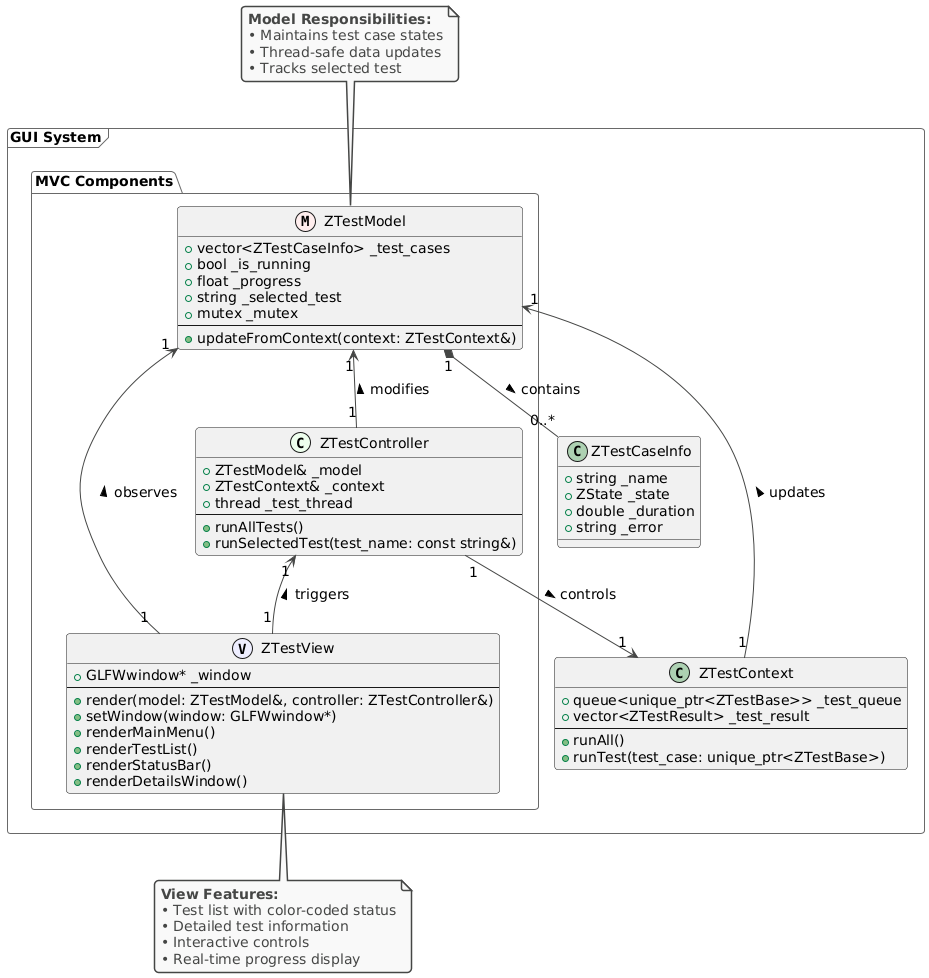
\includegraphics[angle=270,width=\textwidth]{img/umlgui.png} % Insert image
    \caption{ GUI class diagram}
    \label{fig:diagram}
\end{figure}
\begin{figure}[H]
    \centering
    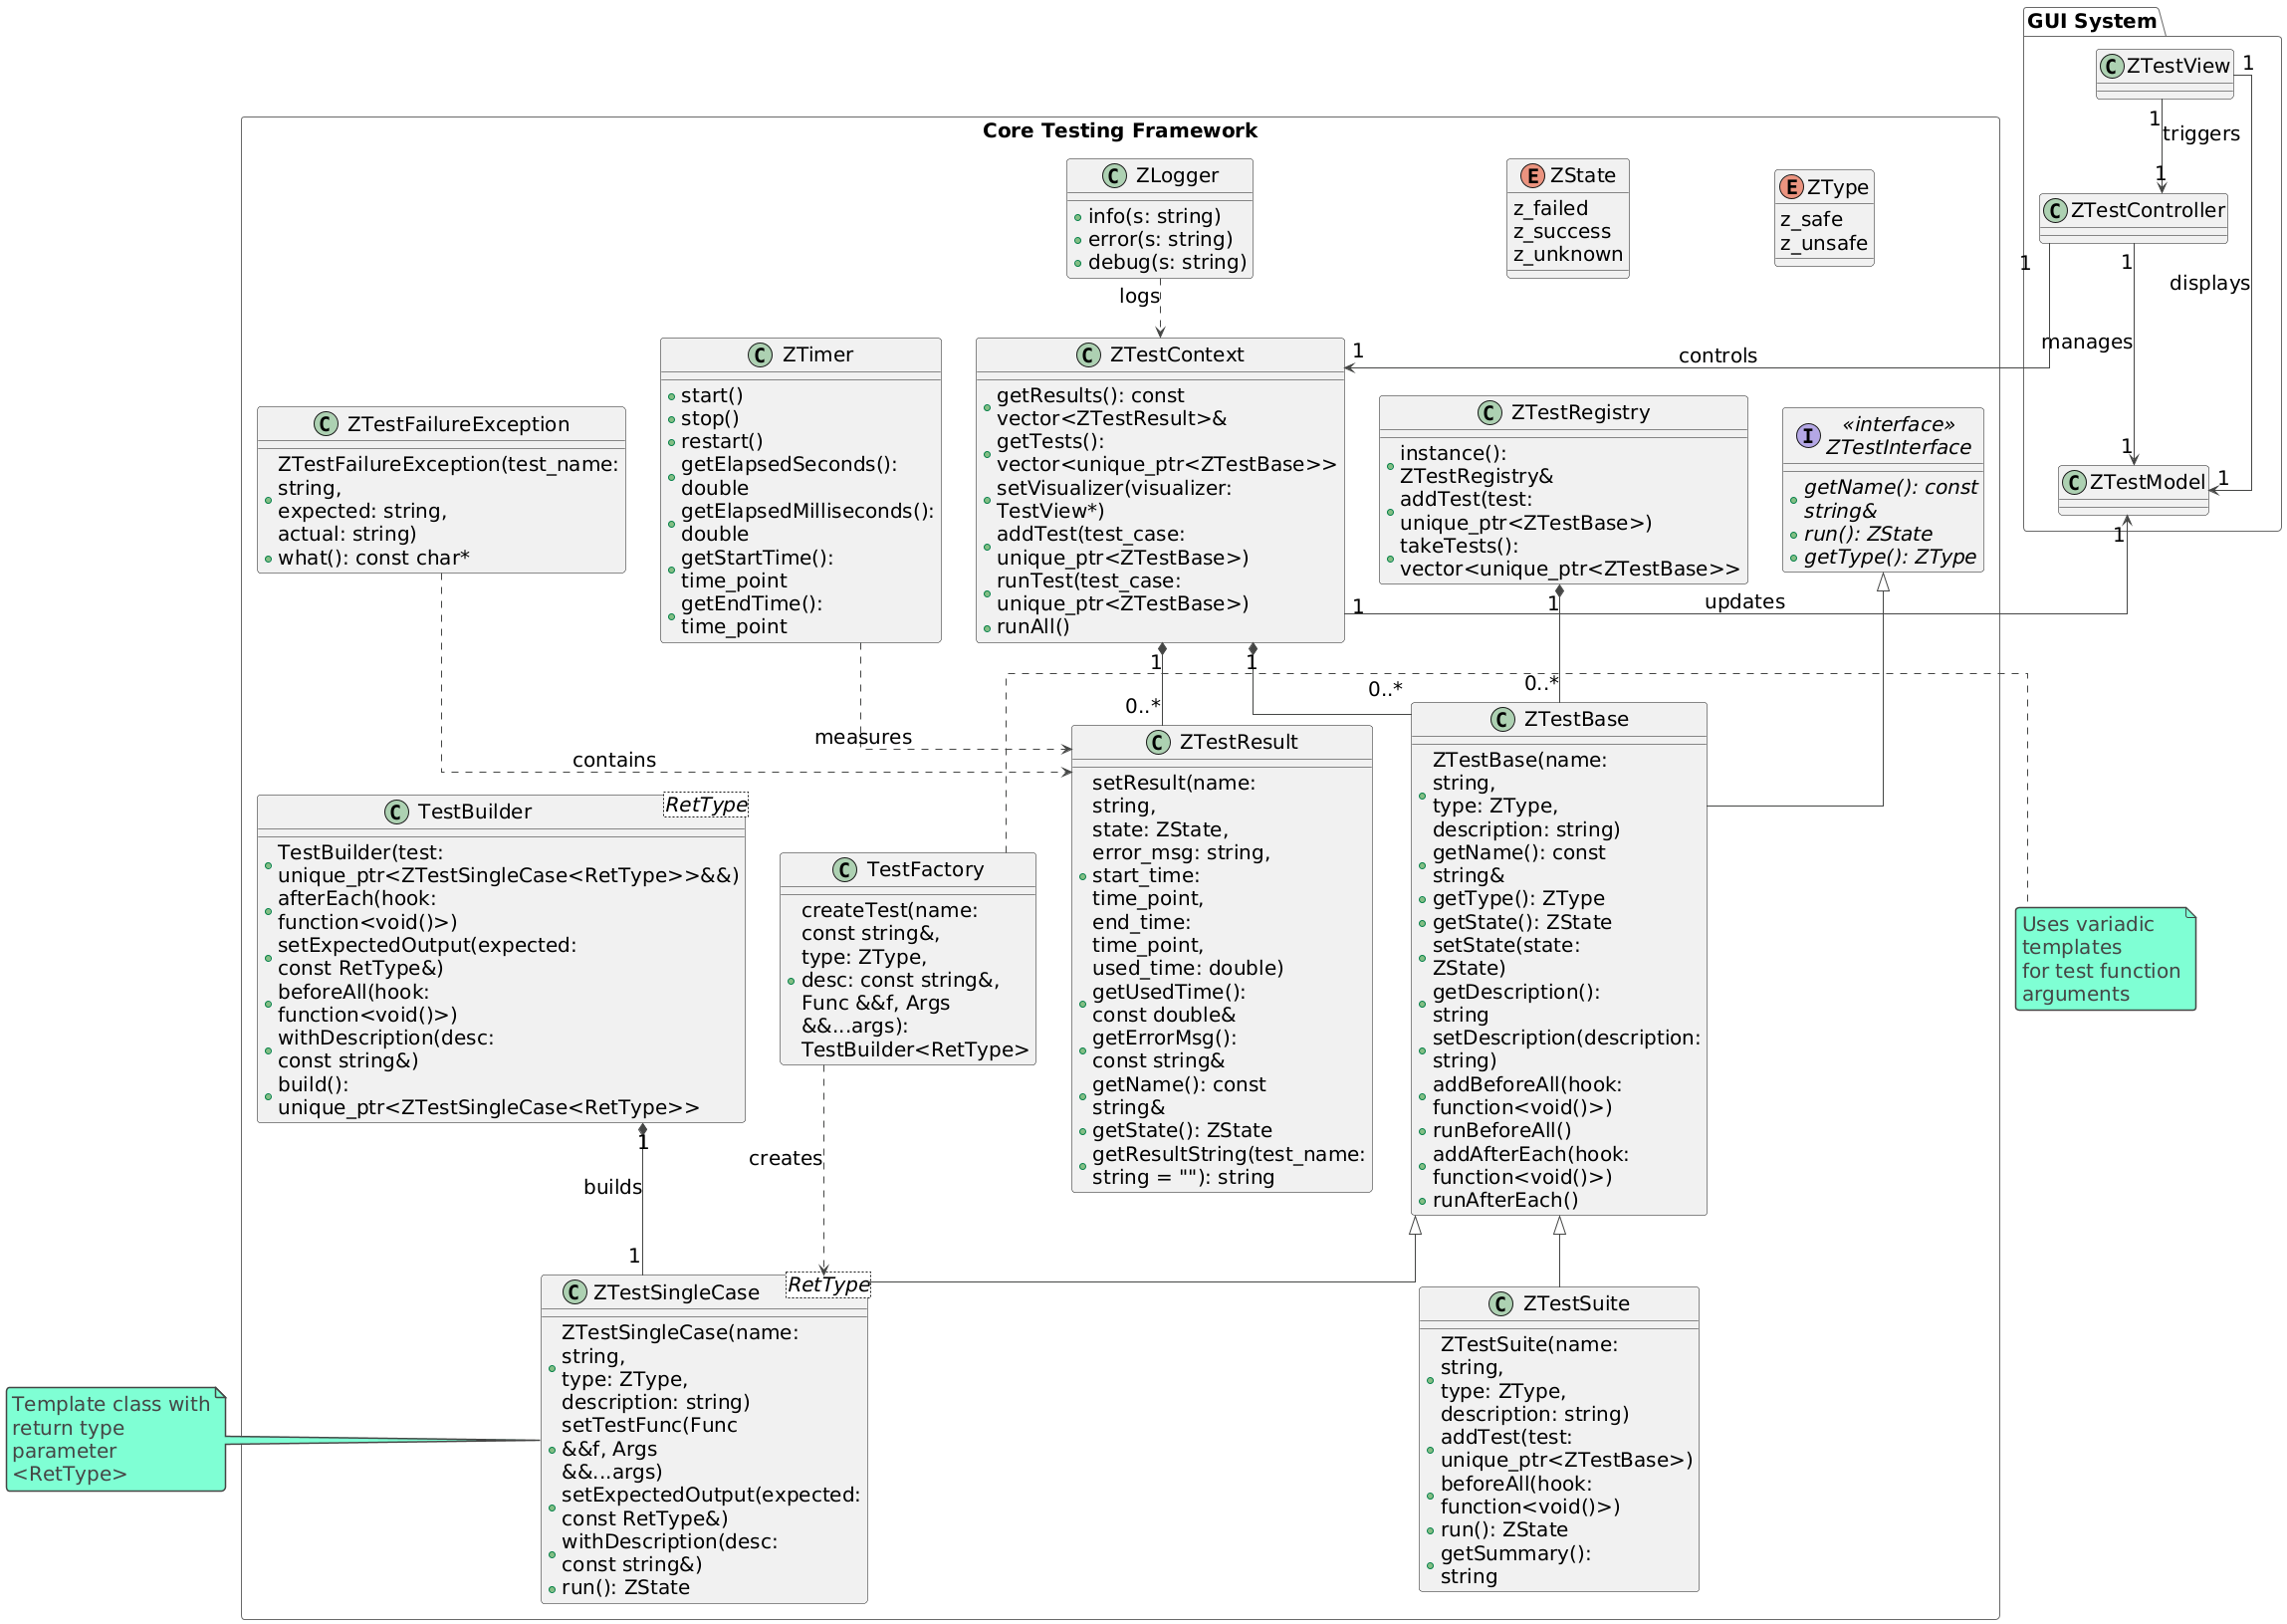
\includegraphics[angle=270,width=0.95\textwidth]{img/umlcore.png} % Insert image
    \caption{ UML class diagram}
    \label{fig:diagram}
\end{figure}

\newpage
% \begin{figure}[H]
%     \centering
%     \includegraphics[angle=270,width=0.88\textwidth]{img/UI.png} % Insert image
%     \caption{UI  class diagram}
%     \label{fig:UI diagram}
% \end{figure}

\subsection{Key Issues for System}
\subsubsection{Automatic Type Inference for Functions to be Tested}
When using \textbf{ZtestSingleCase}, users only need to provide the function name, parameters, and expected result, and \textbf{ZtestSingleCase} will take over the specific logic of running the test and comparing the test results. This requires us to implement automatic inference of the parameter types and return type of the function to be tested when constructing \textbf{ZtestSingleCase}, so that the function can be called for testing and result verification. This is mainly achieved using templates and closures.
\subsubsection{Separation and Dynamic Loading of Files to be Tested and Test Files}
In simple tests, not separating the files to be tested and test files may not seem like a big issue. However, as the size of the project being tested increases and the number of test cases grows, maintaining and modifying the code will become very cumbersome if they are not separated. As a testing framework, we need to provide the ability to separate test files and files to be tested, placing test files in the \textbf{test} folder and files to be tested in the \textbf{src} folder.

We designed our GUI testing framework to act as the main program, while the user's code to be tested and test cases act as plugins. We need to provide an interface \textbf{ZTestAPI} to allow the main program to call functions in the plugins (functions in both test files and files to be tested).
\begin{figure}[H]
    \centering
    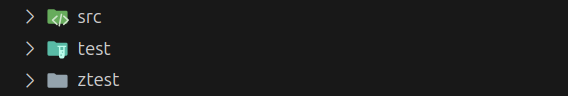
\includegraphics[width=\textwidth]{img/file.png} % Insert image
    \caption{ Directory File Structure}
    \label{fig:diagram}
\end{figure}
\begin{lstlisting}[language=C++]
// Example of exporting a function to be tested
ZTestAPI int subtract(int a, int b) { return a - b; }
\end{lstlisting}
\subsubsection{Implementation of Multiple Construction Methods}
Implementing multiple test case construction methods is actually aimed at providing a better user experience. In terms of implementation, chain creation mainly uses the Builder design pattern, individual test case creation mainly uses the Factory pattern, and macro definition mainly expands to inheritance definition. The implementation of multiple syntaxes facilitates users, but how to manage these syntax-constructed classes uniformly is a challenge.
\begin{figure}[H]
    \centering
    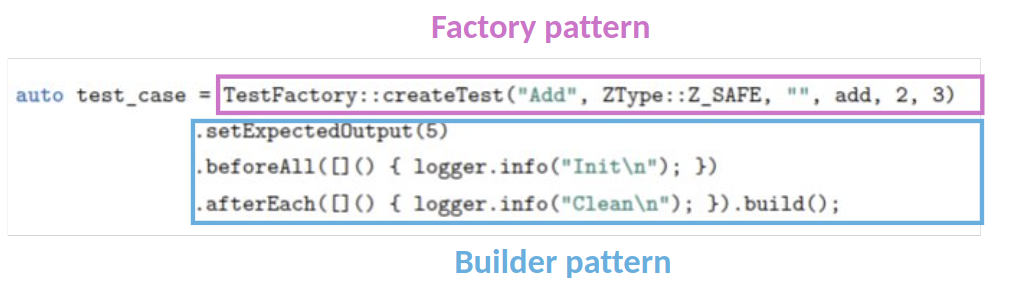
\includegraphics[width=0.8\textwidth]{img/build.png} % Insert image
    \caption{ Implementing Chain Creation}
    \label{fig:diagram}
\end{figure}
\subsubsection{Safe Multi-threaded Evaluation}
Not all functions are thread-safe. Therefore, we need to categorize the functions to be tested and perform thread-safe evaluation accordingly. There are actually two types of test cases that can be defined: \textbf{z\_safe} and \textbf{z\_unsafe}. These two types correspond to two testing modes. \textbf{z\_safe} test cases are thread-safe, while \textbf{z\_unsafe} test cases are not thread-safe. The default type is \textbf{z\_safe}.

If \textbf{z\_unsafe} types appear during testing, the framework will wait for their execution to complete before running \textbf{z\_safe} test cases.
\begin{figure}[H]
    \centering
    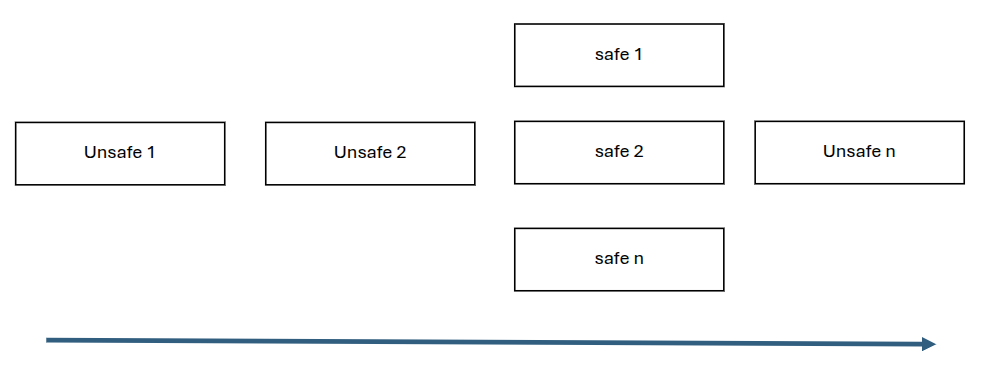
\includegraphics[width=\textwidth]{img/run.png} % Insert image
    \caption{ Implementing Safe Multi-threaded Execution}
    \label{fig:diagram}
\end{figure}
\subsubsection{Test Result Data Storage}
After using multi-threaded evaluation, the order of each evaluation may not be the same each time. However, we do not want the results of each evaluation to be displayed in a different order on the GUI. Additionally, we need to store historical test results to enhance user experience. From a design perspective, we should add an intermediate layer, more precisely, we may need to add a database-like module to store test results for use by \textbf{ZTestModel}.
\subsubsection{Pointer Management}
Considering that this framework uses a large number of pointers, memory leaks and other issues can easily occur. Therefore, we decided to use smart pointers in C++11 to manage memory and improve the reliability of the system.
\subsection{Duty Assignment}
\begin{table}[H]
    \centering
    \caption{Assignment Table}
    \begin{tabular}{l>{\centering\arraybackslash}p{5cm}} % First column left-aligned, second column centered
        \toprule % Add top bold line
        \textbf{Functional Module} & \textbf{Responsible Person} \\ % Add header
        \midrule
        GUI Implementation         & Wu Hongqing                 \\
        Assertion Mechanism        & Wang Ruiqing                \\
        Test Case Management       & Zheng Chenyang, Ye Suohua   \\
        Test Case Execution        & Zheng Chenyang              \\
        Report Result Generation   & Qi Yansong                  \\
        \bottomrule % Add bottom bold line
    \end{tabular}
\end{table}
\subsubsection*{GUI Implementation}
\begin{itemize}[leftmargin=1em,itemsep=0.5ex]
    \item Developed a visual interface based on the Dear ImGUI framework.
    \item Implemented a three-column layout for the test list (name/status/duration).
    \item Developed progress bar components and real-time status bar updates.
    \item Implemented error message rendering for the test details window.
\end{itemize}

\subsubsection*{Assertion Mechanism}
\begin{itemize}[leftmargin=1em,itemsep=0.5ex]
    \item Designed type-safe templated assertion macros (EXPECT\_EQ/ASSERT\_TRUE).
    \item Implemented colored error output.
    \item Developed an extensible exception handling framework (ZTestFailureException).
    \item Supported the registration mechanism for custom comparison operators.
\end{itemize}

\subsubsection*{Test Case Management}
\begin{itemize}[leftmargin=1em,itemsep=0.5ex]
    \item Built a chained API (TestBuilder) to implement a fluent interface.
    \item Developed a macro expansion system (ZTEST\_F) for automatic registration.
    \item Designed a tree-shaped organizational structure for test suites (ZTestSuite).
    \item Implemented dependency injection mechanisms for pre-test and post-test hooks.
    \item Developed a plugin-based test loading system (dynamic library integration).
\end{itemize}

\subsubsection*{Test Case Execution}
\begin{itemize}[leftmargin=1em,itemsep=0.5ex]
    \item Built a thread pool scheduler (ZTestContext).
    \item Implemented isolated execution strategies for safe and unsafe tests.
    \item Designed a test priority queue with timeout termination mechanisms.
\end{itemize}

\subsubsection*{Report Result Generation}
\begin{itemize}[leftmargin=1em,itemsep=0.5ex]
    \item Designed a structured result storage format (ZTestResult).
    \item Implemented ANSI escape code-based colored console output.
    \item Built a version comparison system for historical test results.
    \item Integrated data visualization components (chart generation).
\end{itemize}
\newpage
\addcontentsline{toc}{section}{References}
\begin{thebibliography}{99}

    \bibitem{googletest}
    GoogleTest - Google Testing and Mocking Framework.
    \url{https://github.com/google/googletest}.
    Accessed: 2025-04-27.

    \bibitem{junit5}
    JUnit 5 - The 5th major version of the programmer-friendly testing framework for Java and the JVM.
    \url{https://github.com/junit-team/junit5}.
    Accessed: 2025-04-27.

    \bibitem{pytest}
    The pytest framework makes it easy to write small tests, yet scales to support complex functional testing.
    \url{https://github.com/pytest-dev/pytest}.
    Accessed: 2025-04-27.

    \bibitem{catch2}
    Catch2 - A modern, C++-native, test framework for unit-tests, TDD and BDD.
    \url{https://github.com/catchorg/Catch2}.
    Accessed: 2025-04-27.

    \bibitem{googletestuserguide}
    GoogleTest User’s Guide.
    \url{https://google.github.io/googletest/}.
    Accessed: 2025-04-27.

\end{thebibliography}

\end{document}